\documentclass{scrartcl}
\usepackage{graphicx}
\title{Artificial Intelligence for Robotics (Lab)}
\subtitle{\begin{Large}
Assignment 1
\end{Large}}
\date{\today}
\author{Mihir Patil}

\begin{document}

\maketitle
\pagenumbering{arabic}
\textbf{1. Briefly explain the concepts of reflex-, model-, goal-, and utility-based agents.}\\

\underline{\textbf{Simple Reflex agents-}} Simple reflex agent performs actions based on the current percept received by the agent. It completely ignores the percept history or percept list hence resulting in a small and clean program.It follows a condition-action rule, where the obtained percerpt is matched against a conditon and the corresponding action is executed.\\

\underline{\textbf{Model Based Reflex agents-}} Model based reflex agents are similar to a simple reflex agent but in addition to the current percept they have a model of the unperceptable environment which contains information about how the environment evolves independently of the agent, as well as information about how the agents actions affect the environment.Model based percept agents maintain an internal state based on the percept history.\\

\underline{\textbf{Goal Based agents-}} Goal based reflex agents have in additon to a reflex model a defined goal, which allows them to describe desireable situations. But it differs from a model based agent on the fact that it takes into account the impact of its actions on the future. By answering questions such as "What will happen if i do this?" and "What will make me happy?"\\

\underline{\textbf{Utlity based agents-}} These are simply agents which utilise a utility function to achieve their goal. Utility function is an internalisation of the performance measure which allows the agent to measure its own happiness. And i effect allowing it to achieve its goal with maximum efficiency
\newpage

2. Both the performance measure and the utility function measure how well an agent is doing. What is the difference between the two?\\

While a \textbf{performance measure} helps us evaluate the performance of a agent in an environment, it is imposed on the agent by the designer. And it gives us an idea about whether the agent is doing what it is supposed to do. The performance measure measures the desireability of the environment and tells the agent what it has to do to achieve that desireable state of the environment.\\

On the other hand a \textbf{utility function} is a function internally used by the agent to evaluate its performance. It is used to measure the "happiness" or utility of the agent. Hence it allows the agent to reach the goal or a desireable state in the environment in the most efficient(optimal) way. It is not neccessary for an  agent to have a utility function but it is important for an agent to have a performance measure.\\

In some cases where the utility function and the performance measure end up having the same values, an agent that chooses an action that will have maximum utility will be considered rational with respect to it's external performance measure.

\newpage

3. What is a Braitenberg vehicle? How would you classify Braitenberg vehicles? Are they reflex-, model-, goal-, or utility-based agents?\\
\textbf{Braitenberg vehicles} are simple mobile agents that can move around autonomously,
based on their sensor inputs. In a braitenberg vehicle the sensors are connected directly to the effectors(namely the motors), so that the response time between sensing a signal and reacting to it is greatly reduced. In a braitenberg vehicle the motion of the vehicle is controlled directly by the sensors there is no higher intelligence which models the agent's behaviour based on the percept history.\\

Two sensor-Two actuator Braitenberg vehicles are classified based on their behaviour pattern with respect to a stimuli from the environment. In the case of a light based stimuli the braitenberg vehicles are classified as aggressive(moves towards the light), coward(moves away from the light), love(stares permanently at the light source), explorer(moves towards a light source and then moves away from it to find a brighter source). 

Two Sensor Braitenberg vehicles are simple reflex agents, where the agent doesn't have access to a percept history and modifies its movement based only on the current percept. It doesn't consist of a model which keeps track of the changes in the environment nor does it have a defined goal that can be modified without making any changes to the existing agent program or architecture.


\newpage

4. The missionaries and cannibals problem states: Three missionaries and three cannibals are on the left side of a river, along with a boat that can hold one or two people. The boat cannot move empty, since someone has to row. Find a way to get everyone to the other side, without ever leaving a group of missionaries on one side outnumbered by the cannibals on that side. \\

a). Think of one iteration as the sequence of loading the boat, rowing over the river and unloading the passengers. What information is required to fully describe the state of the problem before/after each iteration? \\

1)The number of missionaries and cannibals on either side of the river at any given point of time.\\

2)The number of cannibals or missionaries in the boat at a given point of time, with respect to the side that the boat is docked.\\


b). Illustrate the complete state-space of the problem as a tree. The root node represents the initial configuration: all six individuals and the boat are on the left side of the river. Each edge represents a shipment of at most two persons to the other side. Add nodes for disallowed configurations, mark them accordingly and do not expand
them further. Is it wise to check for repeated states? Why (not)? \\

It is wise to check for repeated states as the state which has been traversed once need not be traversed again and hence common states can be redirected to follow the common path to traverse to the next node, reducing the time complexity. \\

\begin{figure}
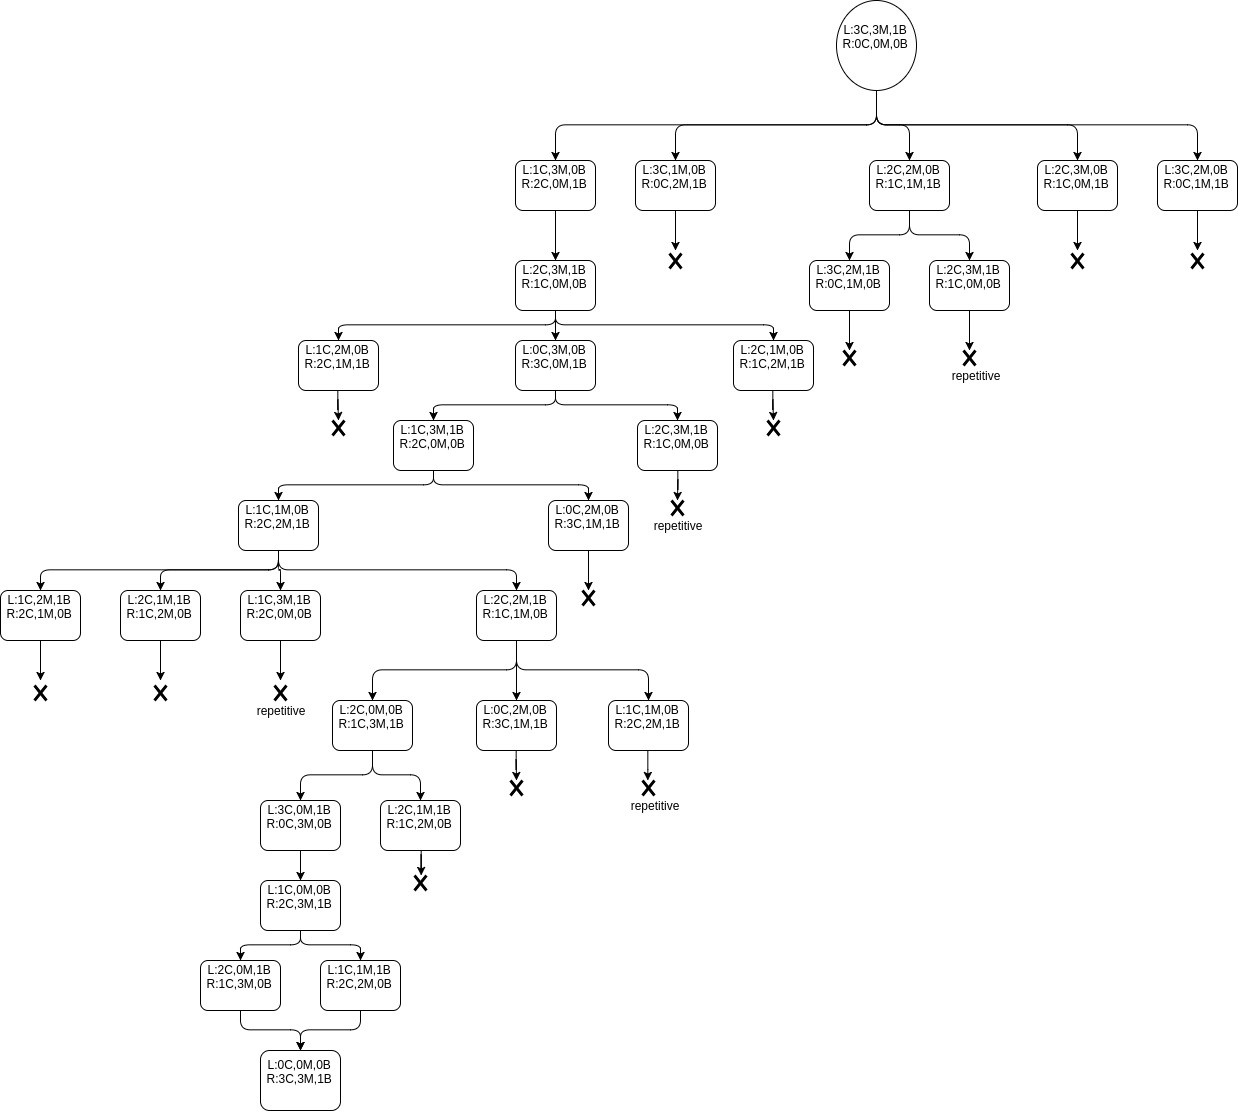
\includegraphics[width=\linewidth]{tree}
\end{figure}


\end{document}

* The illustration of the state-space problem as a tree was completed with help from Sathiya Ramesh.